\chapter{Risiko Analyse}

\section{Hintergrund}
Risikoanalysen dienen dazu vorhersehbaren Risiken zo erkennen, wenn möglich zu beheben und wenn nicht Möglich, wenigstens im Vorhinein zu identifizieren um besser darauf reagieren zu können. Die wesentlichen Schritte zu einer Risikoanalyse lassen sich wie folgt beschreiben.
\begin{figure}[H]
	\centering
	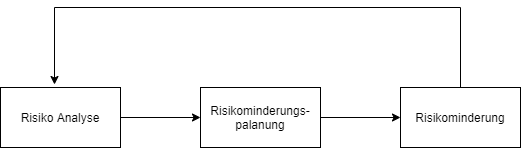
\includegraphics[width=0.8\textwidth]{risk-mitigation-loop}
    \caption{Risikoanalysezyklus \cite{osti_1494012}}
	\label{fig:r1}
\end{figure} 
\subsubsection{Risikoanalyse}
Während der Risikoanalysephase werden mögliche Risiken benannt und strukturiert erfasst und bewertet. Hierfür bieten sich mehrere Techniken an wie z.B das erstellen einer Risiko Matrix. Hierbei werden mögliche Risiken nach ihrer Schwere sowie ihrer Eintrittswahrscheinlichkeit kategorisiert. Ein Risiko welches eine sehr niedrige Eintrittswahrscheinlichkeit hat dafür aber nur sehr unwahrscheinlich eintritt kann unter Umständen akzeptabler sein als eines mit einem geringeren Impact aber einer hohen Eintrittswahrscheinlichkeit.
\begin{figure}[H]
	\centering
	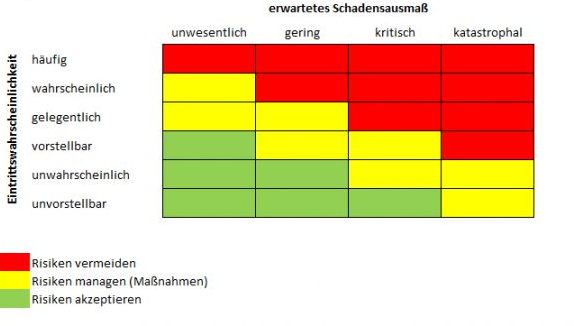
\includegraphics[width=0.8\textwidth]{risk-matrix}
    \caption{Beispiel für eine Risikomatrix \cite{risk2022}}
	\label{fig:r2}
\end{figure} 
\subsubsection{Risikominderungsplanung}
Bei der Risikominderungsplanung wird entschieden wie mit Risiken umgegangen werden soll. Hierbei wird für jedes erkannte Risiko entschieden wie mit ihm umgegangen wird. Mögliche Vorgehensweisen sind:
\begin{itemize}
    \item \textbf{Vermeiden:} Hierbei wird für das gefundene Risiko eine Lösung gefunden und damit das Risiko vermieden. Damit besteht kein weiteres Risiko von dem gefundenen Problem 
    \item \textbf{Verhindern:} Beim Verhindern werden Strategien erdacht, welche dazu führen ein Risiko weitest möglich auszuschließen. Ein gewisses Restrisiko besteht weiterhin und das gefundene Problem sollte in zukünftigen Zyklen weiterhin betrachtet werden. 
    \item \textbf{Akzeptieren:} Das Risiko wird so wie es ist akzeptiert und mit den Folgen wird gelebt. Auch diese Risiken sollten weiterhin verfolgt werden, da in Zukunft eine bessere Strategie für ihre Lösung vorhanden sein könnte.
\end{itemize}
\subsubsection{Risikoverhinderung}
In der Risikoverhinderungsphase werden erkannte Probleme anhand des Planes welcher zuvor erarbeitet wurde behoben.
\\
Abschließend kann wieder am ersten Schritt angefangen werden. Gerade in länger laufenden Projekten ist ein kontinuierliches Risikomanagement empfehlenswert, da sich Risiken im Laufe des Projektes verändern können.

\section{Risikoanalyse für das Projekt}
Aus den User stories und nach Rücksprache im Team haben wir die folgenden Risiken für das Projekt identifizieren können:

\begin{table}[ht]
    \centering
    \begin{adjustbox}{width=1\textwidth}
    \small
    \begin{tabular}{|l|l|l|l|}
    \hline
    Risiko & 
    Eintrittswahrscheinlichkeit & 
    Impakt  & 
    Strategie \\ 
    \hline
    Krankheit von Teammitgliedern 
    & Mittel - Hoch 
    & Hoch   
    & \tabitem Aufgaben verteilen \\
    &&&\tabitem Unabhängig voneinander arbeiten \\ 
    \hline
    Integration in SPMS schwieriger als gedacht 
    & Niedrig - Mittel 
    & Mittel 
    & \tabitem Proaktiv auf Hr. Schulz zugehen \\
    &&&\tabitem Frühzeitig testen           \\ 
    \hline
    Kommunikation mit Dozent schwierig                 
    & Niedrig 
    & Niedrig 
    & Proaktiv auf Dozentin zugehen\\ \hline
    Erwartung der Test User nicht erfüllt
    & Niedrig                     
    & Hoch    
    & \tabitem Nutzer frühzeitig involvieren \\
    &&&\tabitem Feedback einholen \\
    &&&\tabitem Fragebogen         
    \\ \hline
    Zeitlicher Aufwand unterschätzt                     
    & Mittel                      
    & Hoch    
    & \tabitem Möglichst genau Planen \\
    &&&\tabitem Erfahrung von Teammitgliedern nutzen \\ \hline
    Aufwand der Implementierung aller Features zu hoch & Mittel                      
    & Mittel  
    & Abestufte Funktionalität einplanen                            
    \\ \hline
    Atomkrieg mit anschließender Zombieapokalypse      
    & ... hoffentlich niedrig?    
    & Hoch    
    & Duck \& Cover \\ \hline
    \end{tabular}%    
\end{adjustbox}
    \caption{Risikoanlyse des Projekts}
    \label{tab:risk-table}
    \end{table}

Aufgrund der überschaubaren Risiken haben wir eine kombinierte Darstellung aus erkannten Risiken, ihren Eintrittswahrscheinlichkeiten und ihrer Lösung, sofern vorhanden, gewählt. Je nach Größe oder Kritikalität eines Projektes können sich separate Darstellungen oder gar Dokumente besser eignen da sie unter Umständen hunderte Risiken enthalten können.